\pdfminorversion=4
\documentclass{beamer}
\usepackage[ngerman]{babel}
\usepackage[utf8]{inputenc}
\usepackage{graphicx}
\usetheme{Warsaw}
\title{Mit Kryptographie die Welt retten}
\subtitle{Cypherpunk in Theorie und Praxis}
\author{Sebastian Beschke \\ \texttt{sebastian@sbeschke.de}}
\institute{Chaostreff Tübingen}
\date{01. 10. 2011}
\begin{document}

\begin{frame}
\titlepage
\end{frame}


\begin{frame}
	\frametitle{Überblick}
	\tableofcontents
\end{frame}

\section{Einführung in die Public-Key-Kryptographie}
\subsection{Geheimschrift}

\begin{frame}
\frametitle{Eine einfache Chiffre}
\begin{columns}

\column{0.5\textwidth}
	\texttt{FBSKHUSXQNV ZULWH FRGH}

\pause	\texttt{cypherpunks write code}

\column{0.5\textwidth}
\pause	\(K=3\)

	\textit{Schlüssel}

\end{columns}
\end{frame}

\begin{frame}
\frametitle{Symmetrische und asymmetrische Verschlüsselung}
\begin{columns}

\column{0.5\textwidth}
	\textbf{Symmetrisches Verfahren:}
	
	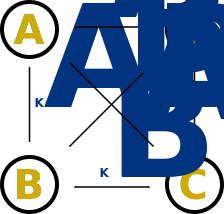
\includegraphics[width=0.9\textwidth]{images/symmetric.pdf}\\

	\small{Verschlüsselung und Entschlüsselung mit gleichem Schlüssel}

	\(\frac{n(n-1)}{2}\) Schlüssel

\pause
\column{0.5\textwidth}
	\textbf{Asymmetrisches Verfahren:}

	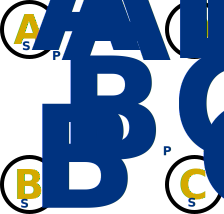
\includegraphics[width=0.9\textwidth]{images/asymmetric.pdf}\\

	\small{Verschlüsselung mit öffentlichem Schlüssel; Entschlüsselung mit privatem Schlüssel}

	\(2n\) Schlüssel

\end{columns}
\end{frame}

\subsection{Das RSA-Verfahren}

\begin{frame}
\begin{itemize}
	\item Das RSA-Verfahren\dots
	\begin{itemize}
		\item Eines der ältesten Public-Key-Verfahren (1978)
		\item Wird noch heute eingesetzt
		\item Basiert auf der Modulo-Rechnung
	\end{itemize}
\end{itemize}
\end{frame}

\section{Privatsphäre unter Beschuss}

\begin{frame}
\end{frame}

\section{Die Anonymisierungssoftware Tor}

\begin{frame}
\end{frame}

\end{document}
